\documentclass[12pt,a4paper]{report}
\usepackage[T1]{fontenc}
\usepackage{ae,aecompl}
% support for images
\usepackage{graphicx}
\usepackage{setspace}
% to modify headers on contents,list of figures ...
\usepackage{fancyhdr}
\usepackage{natbib}
\usepackage{mathptmx}
% support code listings
\usepackage{listings}
% to set page margins
\usepackage[top=2.5cm,bottom=2.5cm,right=2.5cm,left=2.5cm]{geometry}	
\usepackage{ragged2e}
\usepackage{setspace}
\usepackage[raggedright]{titlesec} % to overide default chapter format
\usepackage{sectsty}
%\sectionfont{\bfseries\Large\raggedright}
% for place holder paragraphs
\usepackage{lipsum}

\usepackage{tocloft}
% \usepackage{hyperref} Was giving me more errors than what i was fixing
 
\usepackage{caption}
\usepackage{prettyref}

\usepackage{tabto}
\usepackage{appendix}

\newcommand{\bigtab}{} 
\renewcommand{\figurename}{Fig.}
\newrefformat{fig}{Fig. \ref{#1}}


% Overiding some default headings
\renewcommand{\abstractname}{\normalfont\Large\bfseries ABSTRACT}

% Modify Table of contents to include table header to the top 
\renewcommand*\contentsname{\centering \vspace{-3cm}  \textbf{\Large CONTENTS}
 \\ \vspace{1.2cm} \normalsize Contents \hfill Page No. \par \vspace{-1cm}}

% We do the same for the table of figures too 

\renewcommand{\listfigurename}{\centering \vspace{-3.5cm}\textbf{\Large LIST OF FIGURES} \\ \vspace{.5cm} \normalsize \hspace{.4cm} No.\hfill
  Title\hfill
  Page No. \par \vspace{-1cm}}
  
% Table of tables have the same fate too
\renewcommand{\listtablename}{\centering \vspace{-3.5cm}\textbf{\Large LIST OF TABLES} \\ \vspace{.5cm} \normalsize \hspace{.4cm} No.\hfill
  Title\hfill
  Page No. \par \vspace{-1cm}}
 


\renewcommand{\cftchappresnum}{\chaptername \space}
\addtolength{\cftchapnumwidth}{2cm}
\renewcommand{\cftdot}{}


% Overiding default chapter format
\titlespacing*{\chapter}{0pt}{-40pt}{30pt}
\titleformat{\chapter}[display]
    {\normalfont\Large\bfseries\filcenter}
    {CHAPTER \thechapter}{1pt}{\LARGE}
\titleformat{\section}[display]
    {\normalfont\large\bfseries\raggedright}
    {\thechapter}{1pt}{\large}
    
    % Move it to README or let it be here?
% Report contnet starts from here
%	The sectiong is 
%		\chapter{chapter}
% 		\section{section}
% 		\subsection{subsection}
% 		\subsubsection{subsubsection}
% 		\paragraph{paragraph}
% 		\subparagraph{subparagraph}

 % number of levels to show in ToC, set till paragraph
\setcounter{tocdepth}{4}

% number of levels to show in content, with numbering
\setcounter{secnumdepth}{4} 

\renewcommand\bibname{REFERENCES} 

% Declare Varaibles here, makes it referencing later, no need of changing every place it is used

% To add a new variable the syntax would be 
%	\def \variablename{variable value}

% Declare some frquently used variables

\def \reptitle{Abcd Efghijklmn Opq Rstuvwxyz}
\def \repauthor{ABCDEFG HIJKLMNO}
\def \repregno{1234567890}
\def \repdegree{Master of Technology}
\def \repbranch{Abcdefgh Engineering}
\def \repstream{Zyxwvu Fedcba}
\def \repcollege{Abcdefgh College Of Engineering}
\def \repplace{Abcdefghijkl}
\def \repsupervisor{Opqrestuvw} 
\def \repuniversity{APJ Abdul Kalam Technological University}
\def \repdate{Month 2019} 

% You can declare your own with format 
%
% \def \<variable name>{<variable value>}
% 
% and use it somewhere in report using 
%
%		

\begin{document}
\makeatletter
% Page numbers shall not be shown on Chapter beginning pages.
\renewcommand\chapter{\if@openright\cleardoublepage\else\clearpage\fi
                    \thispagestyle{empty}%
                    \global\@topnum\z@
                    \@afterindentfalse
                    \secdef\@chapter\@schapter}
\makeatother
%\renewcommand\@dotsep{500}
%\renewcommand{\@dotsep}{10000}

% Beginning of title page, the layout maybe different for every one due to different length of title, college names etc, adjust them changing the vspace values
\begin{titlepage}

\begin{center}
%\vspace{-11.0 cm}
    \textbf{\MakeUppercase{ \Large \reptitle}}
    %\maketitle
    %\thispagestyle{empty}
    \vspace{.5 cm}
    \setstretch{1.9}
    \break
    A PROJECT REPORT \\submitted by\\
    \vspace{0.3 cm}
    \textbf{ \large \repauthor \\
    \repregno }
    \vspace{0.3 cm}

	to \\ The \repuniversity \\ in partial fulfillment of the requirements 		for the award of the Degree \\ of \\ \repdegree \\ In

	\repbranch \\
	
	\vspace{0.4 cm}
	% Adjust spacing here to make logo look good
    
\includegraphics[height=0.4\textwidth]{ktu_logo}\par
	\vspace{0.5 cm}
	\textbf{\Large Department of \repbranch}

	\repcollege
	\break
	\repplace \\
	\repdate 
    
    \vfill
\end{center}

\end{titlepage}

% Bottom of the title page

%Declare the page margins for the report, title page is excluded from this
\newgeometry{top=2.5cm,bottom=2.5cm,right=2.5cm,left=3.75cm}

% Clear ant page numbering and start numbering pages using roman numerals
\clearpage
\pagenumbering{roman}

% Declearation page
% TODO move it to a separate file
\center\textbf{\Large DECLARATION}
\break

\justify 
\setstretch{1.5}I undersigned hereby declare that the project report titled \textbf{\reptitle}, submitted for partial fulfillment of the requirements for the award of degree of \repdegree\, of the \repuniversity, Kerala is a bonafide work done by me under supervision of \repsupervisor. This submission represents my ideas in my own words and where ideas or words of others have been included, I have adequately and accurately cited and referenced the original sources. I also declare that I have adhered to ethics of academic honesty and integrity and have not misrepresented or fabricated any data or idea or fact or source in my submission. I understand that any violation of the above will be a cause for disciplinary action by the institute and/or the University and can also evoke penal action from the sources which have thus not been properly cited or from whom proper permission has not been obtained. This report has not been previously formed the basis for the award of any degree, diploma or similar title of any other University. 

\vspace{5cm} % Modify this to any value that pleases your eyes
\begin{flushleft}                           
Place: \repplace \break
Date: \today 
\hfill \repauthor % Keep the student name on same line but right-justify
\end{flushleft}

\newpage 

% Certificate page
\center\textbf{\large \MakeUppercase{department of \repbranch } \break
\MakeUppercase{\repcollege, \repplace}}


\includegraphics[height=0.3\textwidth]{ktu_logo}\par 

\center\textbf{\Large CERTIFICATE}

\justify
%\setstretch{1.5} 
This is to certify that the report entitled \textbf{\large \reptitle} submitted by \textbf{\repauthor} to the \repuniversity\, in partial fulfillment of the requirements for the award of the Degree of \repdegree\, in \repbranch\,  is a bonafide record of the project work carried out by him under our guidance and supervision.. This report in any form has not been submitted to any other University or Institute for any purpose.

\vfill  % push the rest to the bottom of the page
\noindent
%The first signature box 
\parbox[b]{0.4\linewidth}{% size of the first signature box
    \strut
    \centering  
    ----------\\
    (\repsupervisor) \\
    Asst. Prof., Dept. of 
    \repbranch } 
\hspace{2.5cm} % distance between the two signature blocks 
\parbox[b]{0.4\linewidth}{% ...and the second one
    \strut
    \centering 
    -------- \\[0cm]% This 2cm is the space for the signature under the names
    (PG Cordinator) \\
    Professor, Dept. of 
    \repbranch } 
    \par\vspace{0cm}
    
% Not everyone will be lucky to have Principal as guide,so we need to ass more signature spaces, you need to uncomment specific section for your special cases, I will add 3 and 4 signature cases


\vspace{0.5cm}
\begin{center}
\parbox[b]{0.4\linewidth}{% ...and the third one
    \strut
    \centering 
    \\[2cm]
    Abcdefgh Stuvwyz \\[0cm]% This 2cm is the space for the signature under the names
    (Head of the Department) \\
    Department of \repbranch } 
    \par\vspace{0cm}
\end{center}
\newpage

% TODO adjust for external any other certificates, if applicable 
{\centering \textbf{\Large ACKNOWLEDGEMENT} \par }

\addcontentsline{toc}{chapter}{\MakeUppercase{ACKNOWLEDGEMENT}}

%Put in your aknowledgement here
\newpage

% Abstract page

{\centering \textbf{\Large ABSTRACT} \par }
\vspace{.5cm}
\lipsum[1-2]
\addcontentsline{toc}{chapter}{ABSTRACT}

\break
\vspace{-150cm}
\tableofcontents

% List of figures
\newpage
\addcontentsline{toc}{chapter}{LIST OF FIGURES}
\listoffigures 

% List of tables
\newpage
\listoftables
\addcontentsline{toc}{chapter}{LIST OF TABLES}

% List of abbreviations
\newpage
{\centering \textbf{\Large ABBREVIATIONS} \par }
\vspace{.35in}
\noindent
HAS \tab High Altitude Simulation \\
LMTD \tab Logarithmic Mean Temperature Difference \\
PDF \tab Probability Density Function \\

\addcontentsline{toc}{chapter}{\MakeUppercase{Abbreviations}}



% List of notations
\newpage
{\centering \textbf{\Large NOTATIONS}  \par }
\vspace{.25in}
\noindent % Else adds an indent
\break\textit{Latin Symbols} \\
A \tab \tab Area, $m^{2}$ \\
E \tab \tab Voltage, V \\
$R_{e}$ \tab \tab Reynolds number \\
T \tab \tab Temperature, K \\
\break\textit{Greek Symbols} \\
$\alpha$ \tab \tab Diffusivity, $m^{2}\/s$ \\
$\tau$ \tab \tab Shear stress, MPa \\
\break\textit{SuperScripts} \\
2 \tab \tab Square of a number \\
3 \tab \tab Cube of a number \\
\break \textit{Subscripts} \\
hex \tab Hexadecimal Number \\
oct \tab Octal Number

\addcontentsline{toc}{chapter}{\MakeUppercase{Notations}}

% REPORT CONTENT STARTS
\newpage
% Reset Pagenumbers & start arabic numeral numbering for report content
\pagenumbering{arabic}

\chapter{INTRODUCTION}

\section{GENERAL BACKGROUND}

Research is a process of arriving at an appropriate solution to a problem through a systematic approach ………… …………… …………… 
philosophy. 
\\ % Insert break between paragraphs 

There may be various reasons for conducting research. In case of market research more specifically…………………… ……… ………… ………… …… ……
……….. ……… ……… ……… …… ……… …………… ……… ………… ……………
……….. brand. Research is a process of arriving at an appropriate solution to a problem \cite{Dirac}
through systematic approach ……………… ……………… ……………………
……… …………… ………… ………… ………… ………
………… ………… ……………   ..philosophy \citep{mkgandhi}.
\subsection{HISTORICAL BACKGROUND}
 There may be various reasons for conducting research\cite{duncombe}. In case of market
research more specifically  \cite{bradshaw} ………… 
…… ………….. ……… … ………… …………… ………
…………… …… ……… ……… …………… … …….. brand \cite{andrews}.

\subsubsection{GENETIC BACKGROUND ?}
\lipsum[2-4]We need figures for our reports so \prettyref{fig:somelabe} is added below\\ 

\begin{center}    
    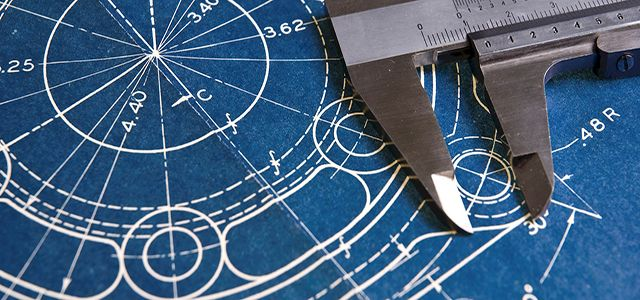
\includegraphics[width=0.8\textwidth]{figures/somename}
    \captionof{figure}{Some random image from Internet}
    \label{fig:somelabe}
\end{center} 

\paragraph{Now I'm just adding section to see how it looks}

\lipsum[1]


\chapter{LITERATURE SURVEY}

%\LARGE{LARGE} vs \Large{LARGE} vs \large{LARGE}
\lipsum[3-8] \\

\lipsum
\chapter{\MakeUppercase{Methodology/Theory/ Modelling}}
\lipsum[1]
% Equatiion are bound to come in reports, so we write one here, found a list of equation at http://www.bbc.com/earth/story/20160120-you-decide-what-is-the-most-beautiful-equation-ever-written
\[(i \partial -m) = 0 \]
Chances are slim your report has a single equation so,
% Eqauations have no captions
\begin{equation}  \label{eq:2}
 f(x) = li(x)-\sum_{\rho}li(x^{\rho}) -  log(2) \frac{dt}{t(t^{2}-1)log(t)}
\end{equation}

Equation \ref{eq:2} is known as Riemann's formula.\lipsum[4]
\chapter{\MakeUppercase{Experimentation}}
\lipsum[1]
\break


\begin{enumerate}
  \item The labels consists of sequential numbers.
  \item The numbers starts at 1 with every call to the enumerate environment.
\end{enumerate}


\chapter{\MakeUppercase{{Results and Discussion}}}
\lipsum[1]
\section{THEORETICAL}
\lipsum[1]The table \ref{table:1} is the same as one provided in the report guidelines. \\
 
\begin{table}[h!]
\centering
\caption{Effect of voltage}
\begin{tabular}{|c | c c | c c|} 
 \hline
 Sl. No. & Voltage & Current & Force & Power \\
  & (V) & (mA) & (N) & (kW) \\
 \hline
 1 & a & - & - & -  \\ 
 2 & - & b & - & - \\
 3 & - & - & c & - \\
 4 & - & - & - & d \\
 \hline
 5 & - & - & - & - \\ 
 \hline
\end{tabular}

\label{table:1}
\end{table}
\section{EXPERIMENTAL}
\lipsum[1]
\chapter{CONCLUSIONS}

After spending a fair amount of time with LATEX, I came to the following conclusions.
\begin{itemize}
  \item This was something I should have learned a few ages ago.
  \item The time I spent with MS word has been the one of the largest waste of my life.
  \item The main idea of this is to show  how a list is prepared.
  \item Well I can write everything I like.Right ?. 
  \item Sometimes you would need a list within a list
  	\begin{itemize}
  		\item An item of the inner list. Let me show you how a citation will look here \cite{grasham1952}
  	\end{itemize}
\end{itemize}

\section{RECOMMENDATIONS}
\lipsum[7-8]
\section{FURTHER STUDIES}
\lipsum[1]

% References page
\newpage
\addcontentsline{toc}{chapter}{\MakeUppercase{References}}

% Set bibliography style , custom style in our case, corresponds to apalikelike.bst file
\bibliographystyle{apalikelike} 

% Load our bibliography file, corresponds to references.bib file
\bibliography{references}

\end{document}
